\subsection{Algorithmic Comparison}

\Cref{tab:full_performance} presents the primary N=32 comparison across five methods, computed from an independently validated evaluation campaign (5 seeds per method, with code and checkpoint hashes verified). This campaign incorporates two isolated, disclosed corrections found during later validation: (i) a units error in the local-compute latency term, where an earlier implementation applied $\log_{10}$ to the local latency component instead of the intended linear term, compressing it toward zero; and (ii) a units error in the Jakes fading Doppler-shift calculation, where carrier frequency was left in GHz rather than converted to Hz, clamping the fading contribution to a numerically negligible floor for LTE and 5G-NR at every realistic vehicle speed. Both corrections were applied as isolated, single-variable patches and validated independently before this campaign was run. $U_{PRR}$ (\Cref{eq:uprr}) is the packet-delivery training signal; $U_{OTR}$ (\Cref{eq:uotr}) is the deadline-compliance criterion. Both are reported for completeness because $U_{PRR}$ forms the training reward and $U_{OTR}$ is recorded during evaluation, but both inherit the unvalidated energy term discussed in the System Model section; the quantitative comparisons below are therefore based primarily on fleet OTR, PRR, latency, and DRR, with $U_{PRR}$/$U_{OTR}$ given alongside as secondary, reward-shaping-derived signals rather than independently validated evidence. At dense fleet scale, MA-ROPE improves over AllOffload on fleet OTR (0.8274 vs. 0.1230) and mean latency (226.5 ms vs. 830.0 ms); the same comparison also holds on the secondary utility signals, $U_{PRR}$ (0.9560 vs. 0.6022) and $U_{OTR}$ (0.5212 vs. 0.1255). CoopEC-RAT is the most competitive alternative, reaching fleet OTR 0.7249 with the lowest mean latency (213.7 ms) among all offloading policies, since its rule offloads only a minority of compute-heavy tasks. UCB-RAT trails both MA-ROPE and CoopEC-RAT on fleet OTR (0.3328). NoOffload achieves fleet OTR $=1.0$ trivially, since it never transmits an offload PDU, and is retained as a reference bound rather than a competitive baseline. NoOffload's $U_{PRR}$, $U_{OTR}$, and latency values are unchanged from the pre-correction campaign to six decimal places, per seed, which is expected: its policy never offloads, so neither correction above applies to any step it takes, and this agreement serves as an internal consistency check on the correction methodology.

\begin{table}[t]
\caption{Full Performance Comparison: URLLC stress, N=32 vehicles, 5 seeds. $U_{PRR}$: Eq. (4a), training signal. $U_{OTR}$: Eq. (4b), deadline compliance. Fleet OTR = on-time offload PDUs / transmitted offload PDUs.}
\label{tab:full_performance}
\centering
% booktabs-restyled
\footnotesize
\setlength{\tabcolsep}{3pt}
\renewcommand{\arraystretch}{1.15}
\begin{tabularx}{\columnwidth}{>{\hsize=2.053\hsize\raggedright\arraybackslash}X>{\hsize=0.789\hsize\raggedleft\arraybackslash}X>{\hsize=0.789\hsize\raggedleft\arraybackslash}X>{\hsize=0.789\hsize\raggedleft\arraybackslash}X>{\hsize=0.789\hsize\raggedleft\arraybackslash}X>{\hsize=0.789\hsize\raggedleft\arraybackslash}X}
\toprule
\textbf{Method} & \textbf{U\_PRR} & \textbf{U\_OTR} & \textbf{Fleet OTR} & \textbf{PRR} & \textbf{Latency (ms)} \\
\midrule
\textbf{MA-ROPE Full \textasteriskcentered} & \textbf{0.9560} & \textbf{0.5212} & \textbf{0.8274} & \textbf{0.9380} & \textbf{226.5} \\
AllOffload (5G 100\%) & 0.6022 & 0.1255 & 0.1230 & 0.9643 & 830.0 \\
NoOffload (local) & 0.9610 & 0.5079 & 1.0000 & 1.0000 & 233.7 \\
UCB-RAT & 0.8871 & 0.4852 & 0.3328 & 0.9627 & 304.6 \\
CoopEC-RAT & 0.9329 & 0.5282 & 0.7249 & 0.9681 & 213.7 \\
\bottomrule
\end{tabularx}
\end{table}


\begin{figure*}[htbp]
\centering
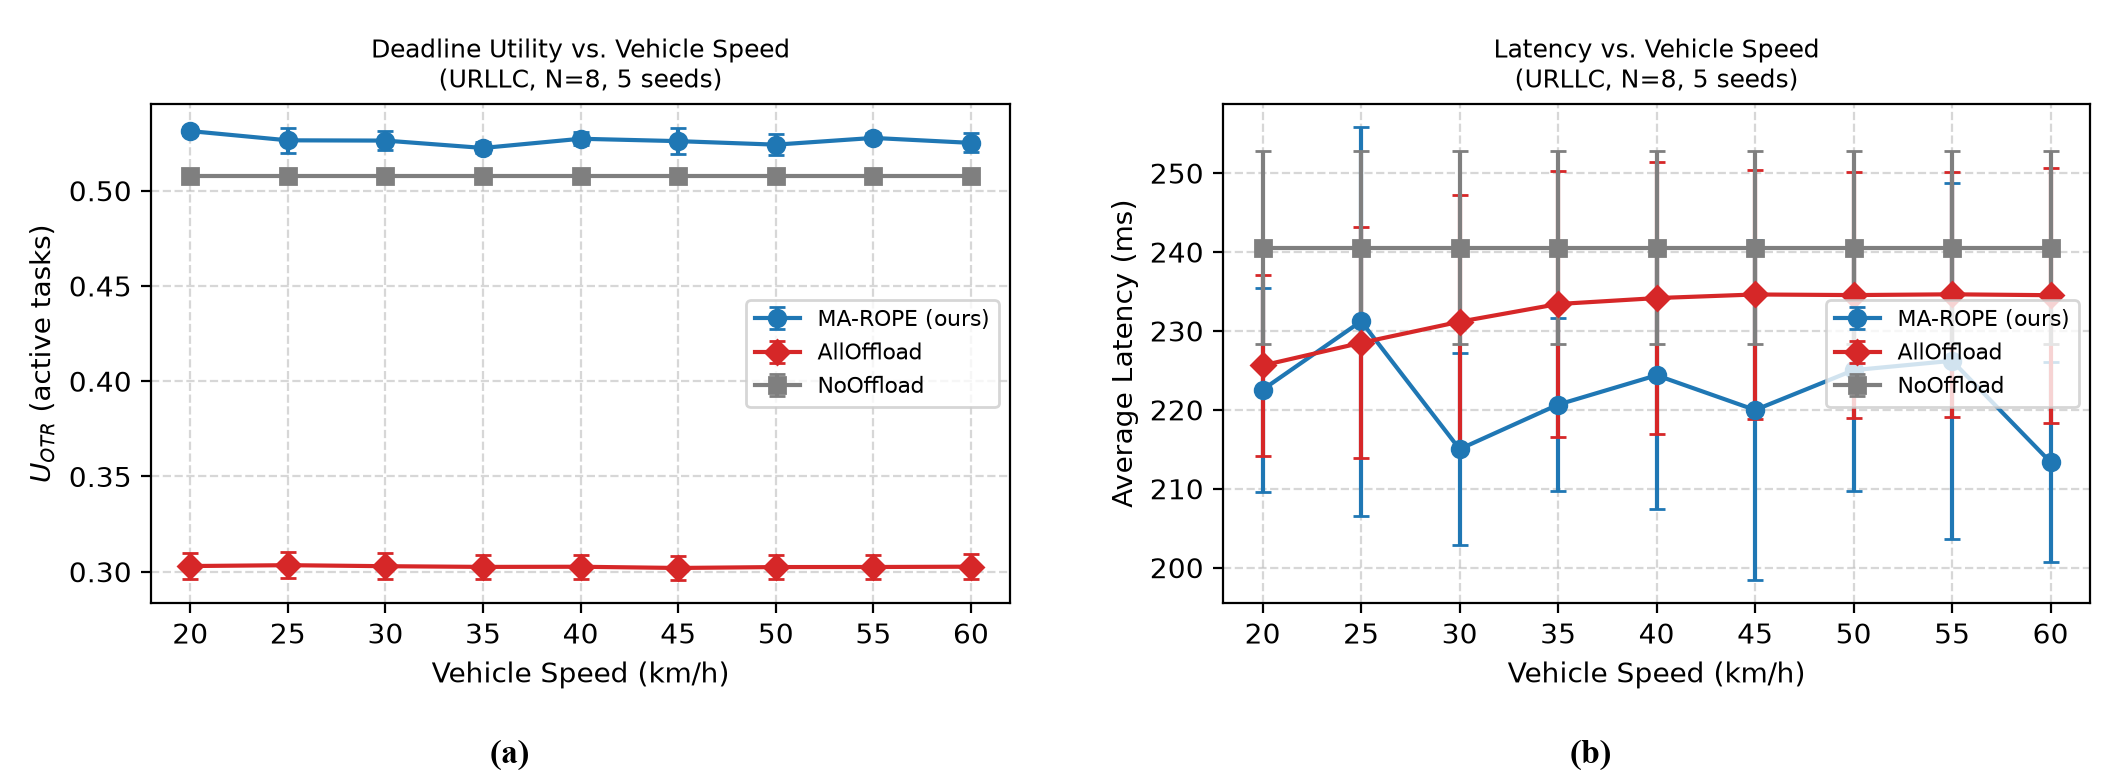
\includegraphics[width=\textwidth]{figures/image5_6_combined.png}
\caption{(a) Deadline utility ($U_{OTR}$, active tasks) and (b) average latency vs. vehicle speed, URLLC scenario, N=8 reference fleet, 5 seeds. MA-ROPE and NoOffload substantially outperform AllOffload on deadline utility across the full 20--60 km/h range, with no strong speed-dependent trend at this fleet size; error bars in (b) show cross-seed standard deviation.}
\label{fig:utility_speed}
\end{figure*}

\begin{figure}[htbp]
\centering
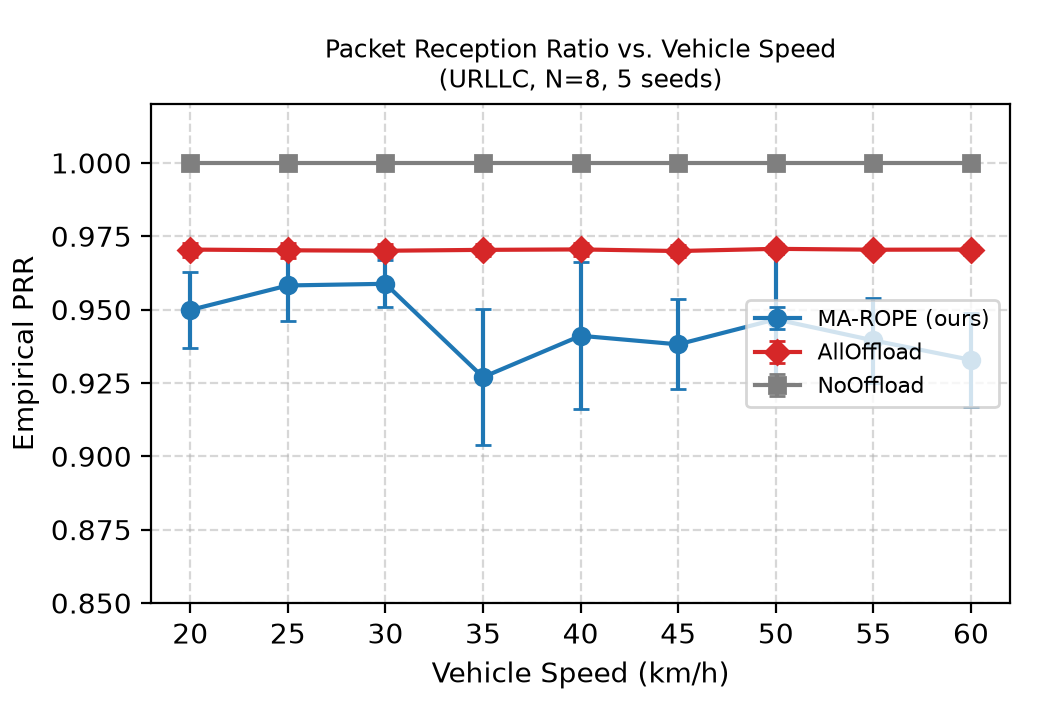
\includegraphics[width=\columnwidth]{figures/image8.png}
\caption{Empirical PRR = $n_{rx}/n_{tx}$ vs. vehicle speed, URLLC scenario, N=8 reference fleet, 5 seeds. All three methods remain above 0.92 across the evaluated speed range.}
\label{fig:prr_speed}
\end{figure}

\subsection{Safety-Critical Task Delivery}

\Cref{tab:safety_task} isolates delivery performance for safety-typed PDUs (100 ms deadline class) at N=32, computed directly from the same validated checkpoints as \Cref{tab:full_performance}, filtered to safety-task transmissions only. The comparison is restricted to MA-ROPE and AllOffload because a validated safety-task-only breakdown is not yet available for UCB-RAT or CoopEC-RAT; extending it to those baselines is left for future work.

\begin{table}[h!]
\caption{Safety-Task Delivery at N=32: Safety PRR and Safety OTR, 5 seeds}
\label{tab:safety_task}
\centering
\resizebox{\columnwidth}{!}{%
\begin{tabular}{|l|r|r|r|}
\hline
\textbf{Method} & \textbf{Safety PRR} & \textbf{Safety OTR} & \textbf{PRR-OTR gap} \\
\hline
\textbf{MA-ROPE Full \textasteriskcentered} & \textbf{0.9317} & \textbf{0.7537} & \textbf{17.8\%} \\
AllOffload & 0.9654 & 0.0000 & 96.5\% \\
\hline
\end{tabular}%
}
\end{table}


At N=32, AllOffload's mean active-task latency (830.0 ms, \Cref{tab:full_performance}) exceeds the 100 ms safety deadline on essentially every attempt, so despite a high link-level Safety PRR (0.9654), zero safety PDUs arrive on time in any of the five evaluated seeds. MA-ROPE's queue- and RAT-aware policy keeps Safety OTR at 0.7537 under the same dense-fleet conditions, and it remains the sharpest illustration in this paper of why PRR alone cannot certify deadline-compliant delivery for safety-critical V2X traffic.

\subsection{Fleet-Density Scaling and RSU Queue Contention}

\Cref{tab:why_marope_wins} summarizes deadline compliance, deadline utility, link failure rates, and step overhead across the validated N=8/16/32 density sweep. The fleet sweep shows the central scaling effect: AllOffload's fleet OTR falls from 33.5\% at N=8 to 12.3\% at N=32, while MA-ROPE remains in the 82-86\% range throughout. MA-ROPE's advantage is large and consistent at every evaluated density, not only at the high end.

\begin{table}[h!]
\caption{Fleet-Density Scaling of Deadline Compliance and Link Reliability (5 seeds)}
\label{tab:why_marope_wins}
\centering
\resizebox{\columnwidth}{!}{%
\begin{tabular}{|l|r|r|l|}
\hline
\textbf{Metric} & \textbf{MA-ROPE} & \textbf{Comparator} & \textbf{Relative Difference} \\
\hline
Fleet OTR @ N=8 & 0.849 & AllOffload 0.335 & +51.3 pp \\
Fleet OTR @ N=16 & 0.861 & AllOffload 0.263 & +59.8 pp \\
Fleet OTR @ N=32 & 0.827 & AllOffload 0.123 & +70.4 pp \\
$U_{OTR}$ @ N=32 & 0.521 & AllOffload 0.126 & +0.396 \\
Fleet-wide link failure @ N=32 & 0.28\% & AllOffload 3.57\% & $\sim$12.8x lower \\
Per-attempt link failure @ N=32 & 6.20\% & AllOffload 3.57\% & 1.7x higher \\
DRR (N=8$\rightarrow$32) & 0.975 & AllOffload 0.367 & 2.66x higher retention \\
Step time & 166.6 \textmu s & Single-RAT 167.6 \textmu s & No penalty \\
\hline
\end{tabular}%
}
\end{table}


\begin{figure}[htbp]
\centering
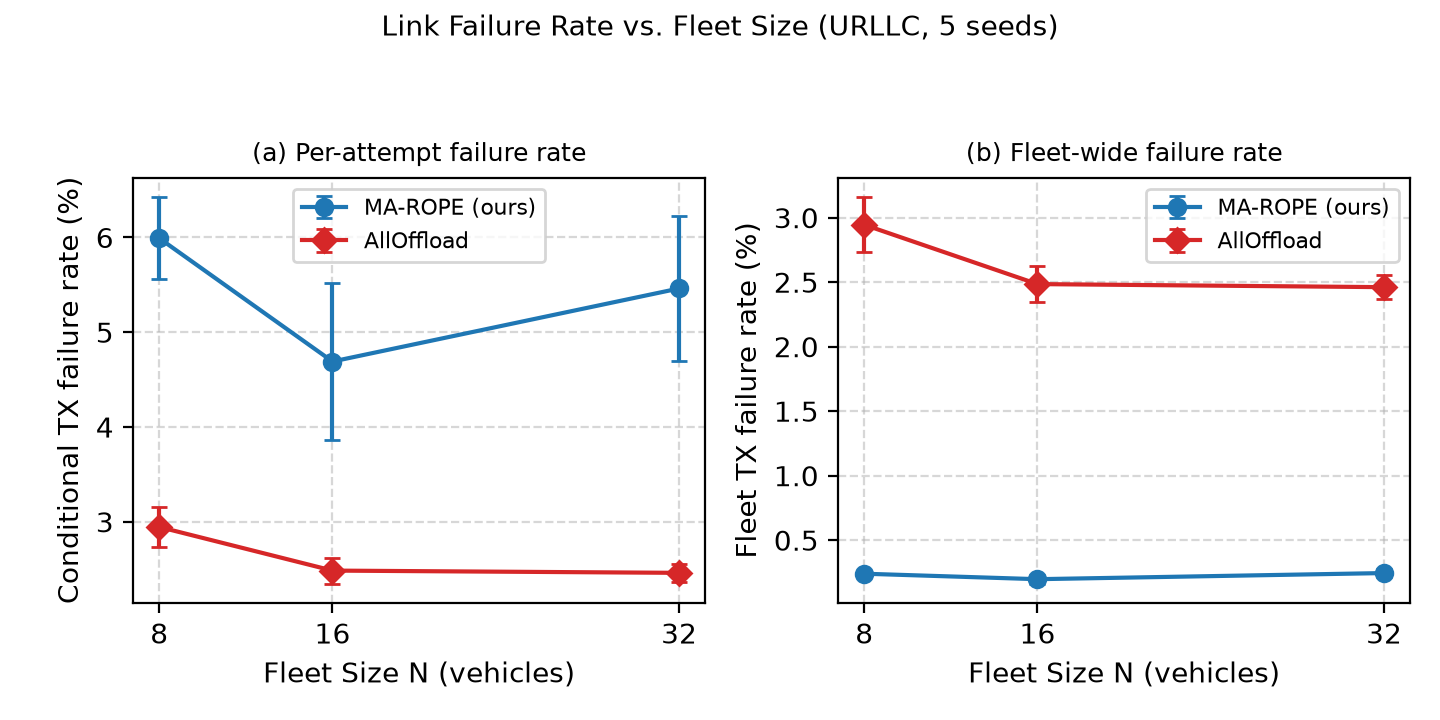
\includegraphics[width=\columnwidth]{figures/image10.png}
\caption{Link failure rate vs. fleet size (URLLC, 5 seeds). (a) Per-attempt failure rate: MA-ROPE's rate is higher than AllOffload's at every density, because MA-ROPE occasionally uses the less reliable WiFi6 link. (b) Fleet-wide failure rate (failures per vehicle-step regardless of whether a transmission was attempted): MA-ROPE remains an order of magnitude below AllOffload at every density, because it transmits far less often. Both metrics are genuine and neither should be read in isolation; see discussion below.}
\label{fig:queue_loss}
\end{figure}

\begin{figure}[htbp]
\centering
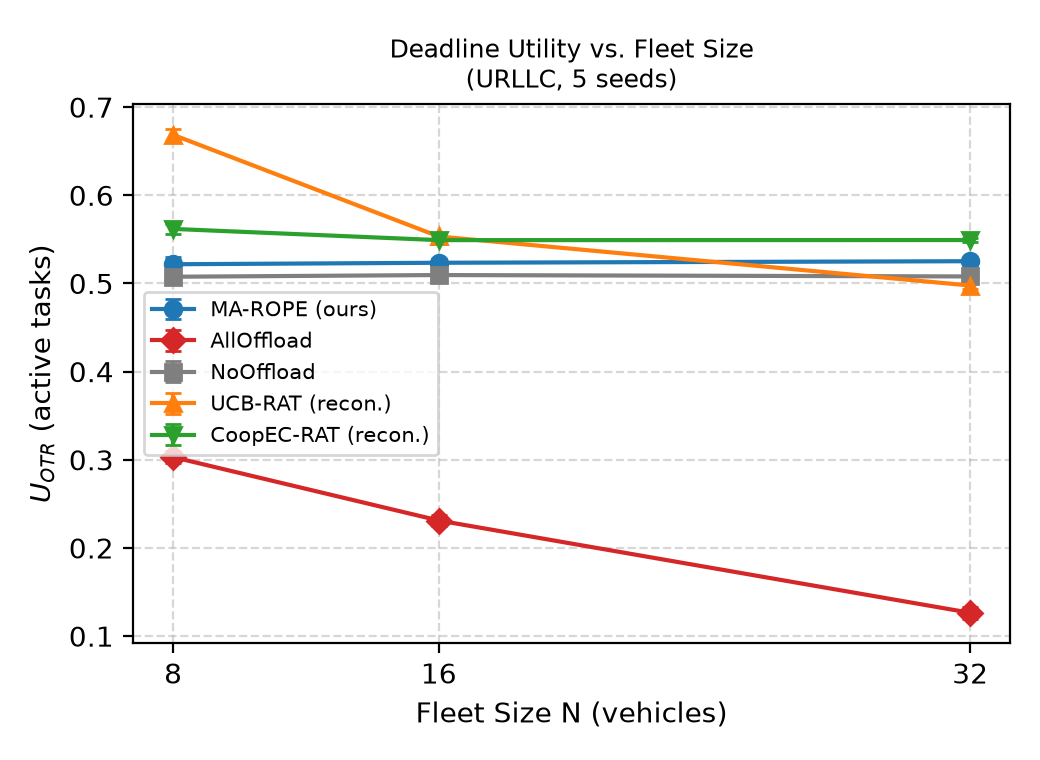
\includegraphics[width=\columnwidth]{figures/image11.png}
\caption{Deadline utility ($U_{OTR}$, active tasks) vs. fleet size (URLLC, 5 seeds). The MA-ROPE-AllOffload utility gap widens from +0.224 at N=8 to +0.396 at N=32.}
\label{fig:system_utility}
\end{figure}

\Cref{fig:fleet_otr} extends the fleet-scaling analysis to on-time delivery. At N=8, MA-ROPE achieves fleet OTR $=0.849$ vs. AllOffload $=0.335$; at N=16 MA-ROPE rises slightly to $0.861$ while AllOffload falls further to $0.263$; and at N=32 MA-ROPE settles at $0.827$ while AllOffload falls to $0.123$. MA-ROPE's density curve is not strictly monotonic: N=16 is marginally higher than N=8, likely within seed-to-seed noise. The overall N=8-to-N=32 trend is a mild decline, and MA-ROPE's degradation is far gentler than AllOffload's at every step.

\textbf{\textit{Deadline Retention under Fleet Density.}} Point-wise OTR characterizes deadline compliance at a particular operating density, but it does not directly express how rapidly that performance deteriorates as the number of competing vehicles increases. We therefore define the Deadline Retention Ratio (DRR) as

\begin{equation}
\text{DRR}(N_{target}, N_{ref}) = \frac{\text{OTR}_{fleet}(N_{target})}{\text{OTR}_{fleet}(N_{ref})}.
\label{eq:drr}
\end{equation}

Here, $N_{ref}$ denotes a reference fleet density and $N_{target} > N_{ref}$ denotes the density at which retention is evaluated. $\text{DRR}=1$ indicates complete preservation of reference-density deadline performance, whereas values approaching zero indicate increasingly severe degradation; values exceeding 1 indicate deadline performance that is actually higher at the target density than at the reference density.

Using $N_{ref}=8$ and $N_{target}=32$, corresponding to a fourfold increase in fleet size, the results in \Cref{tab:why_marope_wins} yield $\text{DRR}(32,8)^{\text{MA-ROPE}} = 0.8274/0.8485 = 0.975$, whereas $\text{DRR}(32,8)^{\text{AllOffload}} = 0.1230/0.3352 = 0.367$. Thus, MA-ROPE preserves approximately 97.5\% of its reference-density on-time delivery performance, whereas single-RAT AllOffload preserves only 36.7\%. At N=16, the corresponding retention values are $\text{DRR}(16,8)^{\text{MA-ROPE}}=0.8611/0.8485=1.015$, slightly exceeding 1 since fleet OTR at N=16 is marginally higher than at N=8 under the corrected physics, and $\text{DRR}(16,8)^{\text{AllOffload}}=0.2634/0.3352=0.786$, showing that MA-ROPE holds essentially complete performance through a doubling of fleet size while AllOffload has already lost more than a fifth of its reference-density delivery rate.

The principal advantage of DRR is normalization. Each policy is evaluated relative to its own reference-density OTR rather than against another method's absolute utility value. Consequently, DRR does not depend on the $\alpha$/$\beta$ weighting or normalization constants used in the MA-ROPE utility formulation and can be applied to other offloading schemes whenever deadline-aware delivery is reported over multiple fleet densities.

\subsection{Discussion}

NoOffload vs. MA-ROPE on composite utility. \Cref{tab:full_performance} shows NoOffload achieving higher $U_{PRR}$ (0.9610) than MA-ROPE (0.9560) at N=32, but NoOffload has no transmitted offload PDUs and fleet OTR is therefore not a meaningful V2X delivery metric for it. The operational claim should therefore be based on fleet OTR, PRR, DRR, latency, and dense-fleet scaling rather than on the composite utility values ($U_{PRR}$/$U_{OTR}$) alone.

Dual utility functions. MA-ROPE exposes two utility criteria: $U_{PRR}$ (\Cref{eq:uprr}) for dense packet-delivery reward shaping and $U_{OTR}$ (\Cref{eq:uotr}) for deadline-compliance-dominant deployment assessment. Conceptually, $U_{OTR}$ is the deadline-aware, safety-facing criterion because a received-but-late safety PDU has zero operational value under 3GPP V2X safety requirements~\cite{molina2017}; as noted above, however, both utility values inherit the unvalidated energy term and are secondary to fleet OTR and DRR, which are this paper's primary safety-relevant evidence. $U_{PRR}$ is reported alongside for balanced and compute-heavy scenarios where throughput dominates over strict timing. Task-adaptive alpha/beta weights are principled rather than tuned: safety alpha=0.70 matches the 65\% safety PDU proportion; compute alpha=0.20 reflects 2000 ms deadline headroom where throughput dominates. A sensitivity analysis of these weights is left for future work.

Link failure rate requires reading two metrics together, not one. MA-ROPE's per-attempt link failure rate (\Cref{tab:why_marope_wins}) is higher than AllOffload's at every evaluated density (6.20\% vs. 3.57\% at N=32), because MA-ROPE occasionally routes traffic over WiFi6, the least reliable of the four supported RATs, when doing so is still utility-optimal overall. Read in isolation, this metric would appear to favor AllOffload. However, MA-ROPE transmits far less often than AllOffload in the first place, by minimizing unnecessary offloading, so its fleet-wide failure rate (failures per vehicle-step rather than per attempt) is an order of magnitude lower (0.28\% vs. 3.57\% at N=32), corresponding to roughly 13x fewer absolute link failures fleet-wide across the evaluated episodes (44.2 vs. 570.6). Reporting both metrics is necessary because the per-attempt measure characterizes conditional link reliability, whereas the fleet-wide measure captures the overall transmission-failure burden of the policy; collapsing them into a single figure would conceal this trade-off.

By trading a higher per-attempt link failure rate for substantially fewer total transmission attempts, substantially higher Fleet OTR scalability, and near-complete deadline-retention under increasing density, MA-ROPE presents a more robust solution for real-world heterogeneous V2X networks under shared RSU contention than a single-RAT policy.

Limitations and future work. \Cref{tab:deadline_analysis} is computed under the same corrected physics as the rest of this section, but at a different fleet size (N=8) and evaluation protocol than \Cref{tab:full_performance} or \Cref{tab:safety_task}, so its absolute figures should not be compared against them directly. The Contribution Decomposition ablation in Section II remains a historical, pre-correction reference and is explicitly disclosed as such where it is presented. \Cref{tab:safety_task} is a two-method N=32 safety comparison (MA-ROPE and AllOffload only); extending it to UCB-RAT and CoopEC-RAT, and reintroducing a validated centralized (MADDPG-style) upper bound, are left for future work. Future work should also evaluate non-IID vehicle/task distributions, secure or differentially private FedAvg, and sensitivity to alpha/beta weights and queue service rates.

\begin{figure}[htbp]
\centering
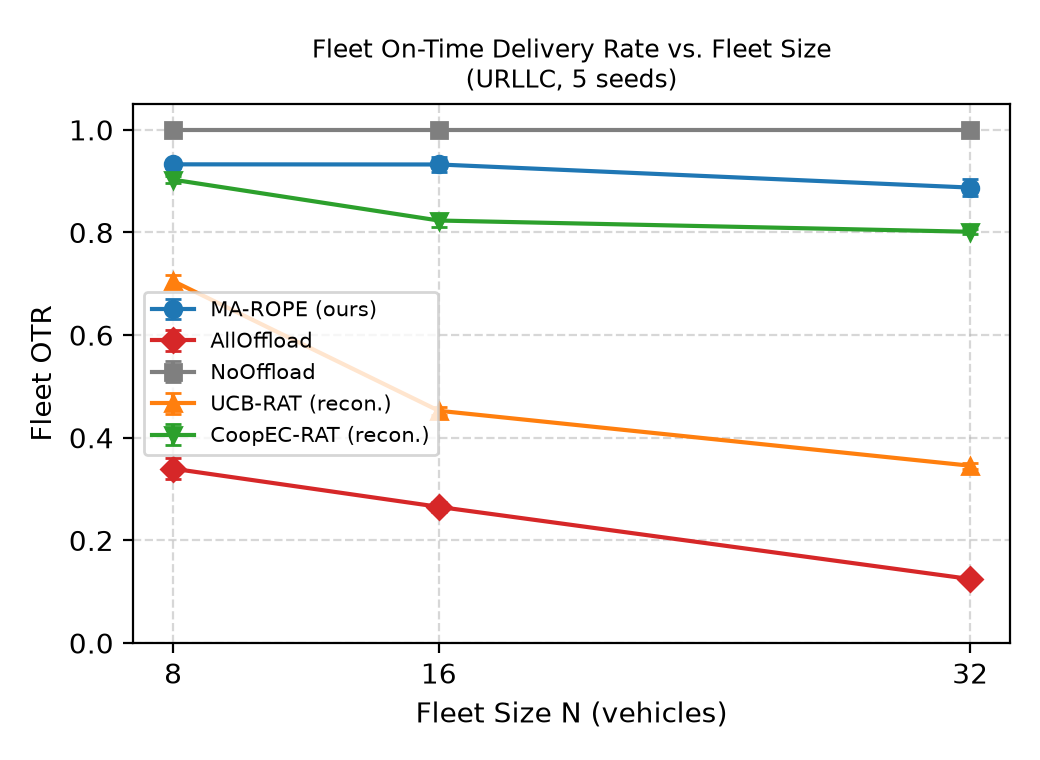
\includegraphics[width=\columnwidth]{figures/image12.png}
\caption{Fleet OTR vs. fleet size (URLLC, 5 seeds). MA-ROPE holds 0.827--0.861 fleet OTR across N=8/16/32, while AllOffload falls from 0.335 at N=8 to 0.123 at N=32.}
\label{fig:fleet_otr}
\end{figure}

The divergence in deadline compliance is large and consistent at every evaluated density, not only at high fleet size. At N=8, MA-ROPE already leads AllOffload by 51.3 percentage points in fleet OTR (0.849 vs. 0.335); by N=16 the gap widens further as AllOffload continues to decline while MA-ROPE holds essentially flat (0.861 vs. 0.263); and at N=32, AllOffload falls to 0.123 while MA-ROPE remains at 0.827. The DRR analysis above points to the same conclusion: MA-ROPE keeps deadline-compliant delivery working at scale, where AllOffload does not.
